% %%%%%%%%%%%%%%%%%%%%%%%%%%%%%%%%%%%%%%%%%%%%%%%%%%%%%%%%%%%%%%%%%%%%%
% %% Background %%
% Sparse Formats
% %%%%%%%%%%%%%%%%%%%%%%%%%%%%%%%%%%%%%%%%%%%%%%%%%%%%%%%%%%%%%%%%%%%%%

\section{Sparse Formats}
\label{sec:bg:sparse_formats}

\lettrine{I}{n} the absence of a compressed format, matrices are stored in fixed size two-dimensional arrays.
With this \gls{dFormat}, elements can be randomly accessed ($\mathcal{O}(1)$), and \gls{seqAccesses} are highly efficient.
The two dimensions are called \glspl{rank} which correspond to the rows and columns.
For matrices, there are thus two variants of the \gls{dFormat}, depending on which \gls{rank} is stored sequentially in memory.
In a \emph{row-wise} (or \emph{row-major}) storage, the elements within the rows are sequential, and conversely for \emph{column-wise} (or \emph{column-major}). 

Sparse matrices contain a very large number of zeros, and to avoid storing these repeated zeros, there exist many compressed formats~\cite{Tewarson1973_COO_CSR_LIL_first, Kincaid1989_ELLPACK, Barrett1994_CSR_BCSR_DIA_ELL, Saad2003_COO_CSR_DIA_ELL, Bell2009_HYB, Chou2018_COO_CSR_DIA_ELL_HASH}, where certain formats are best-suited for matrices with a specific structure.
The main principle of these \glspl{spFormat} is to avoid storing the zero elements, compensating with additional \gls{metadata} which gives the position of the non-zero elements.

We can cite some of the most used \glspl{spFormat} like \acrfull{coo} that uses three tables of size $nnz$ with only the non-zero elements ($val$ table in Figure~\ref{fig:bg:FormatEx:COO}) and their row and column indices ($row$ and $col$ $idx$ tables).
This format is the simplest one.
It does not need to be sorted to be effective which is a great advantage when the data is ``randomly'' updated.
However, it is an inconvenient for matrix sequential traversals or search tasks.
This format can be sorted \emph{row-wise} as in the example in Figure~\ref{fig:bg:FormatEx:COO} or \emph{column-wise} if needed, but would lose its advantage compared to the two mostly used \glspl{spFormat} \acrfull{csr} (Figure~\ref{fig:bg:FormatEx:CSR}) and its \emph{column-major} counterpart \acrfull{csc} (Figure~\ref{fig:bg:FormatEx:CSC}), which are sorted by construction.
With \acrshort{csc}, the $val$ table of size $nnz$ stores the non-zero elements sorted \emph{column-wise} and the $idx$ table of size $nnz$ stores the corresponding row indices, similarly to \acrshort{coo}.
The third table $ptr$ of size $M+1$ stores the positions of the columns.
For example, in Figure~\ref{fig:bg:FormatEx:CSC}, the second column of index $1$ (\textit{green}) has non-zero elements between positions $2$ and $4$ (\textit{blue}, $4$ excluded) of tables $idx$ and $val$.
This $ptr$ table allows \acrshort{csr} and \acrshort{csc} to have a lower memory footprint than \acrshort{coo}.

\begin{figure}[htbp]
    \centering
    \begin{subfigure}[t]{0.32\linewidth}
        \centering
        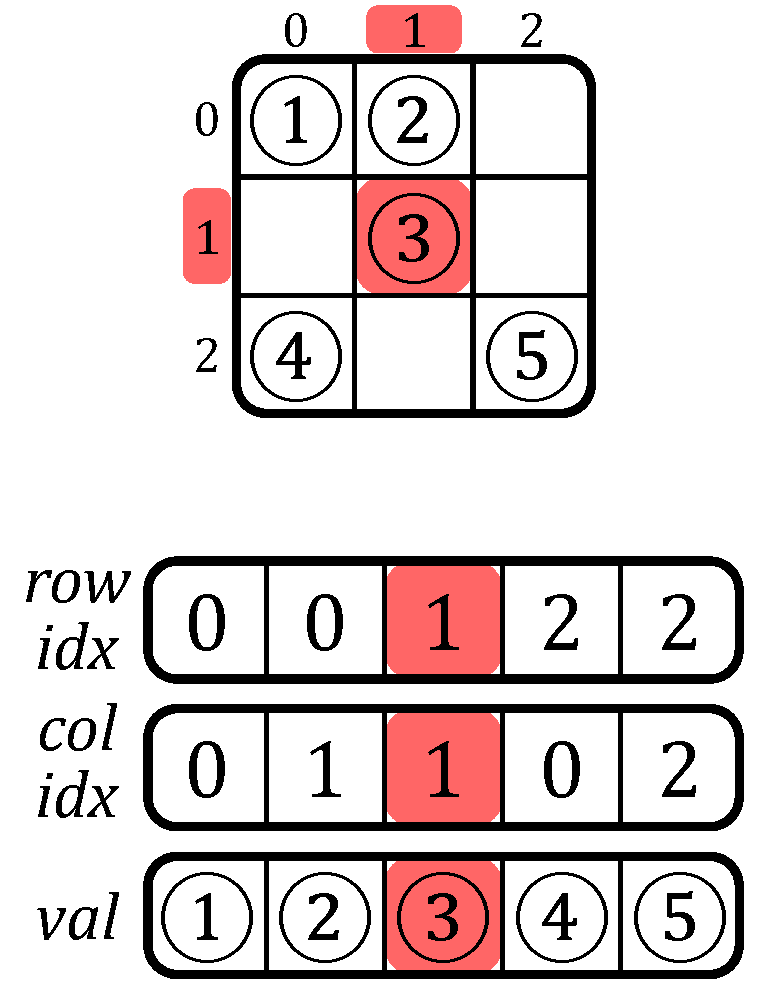
\includegraphics[width=0.8\linewidth]{Chapter_Background/Figures/PDF/SparseFormats/SpFormats_COO.pdf}
        \caption{\acrshort{coo}}
        \label{fig:bg:FormatEx:COO}
    \end{subfigure}
    \hfill
    \begin{subfigure}[t]{0.32\linewidth}
        \centering
        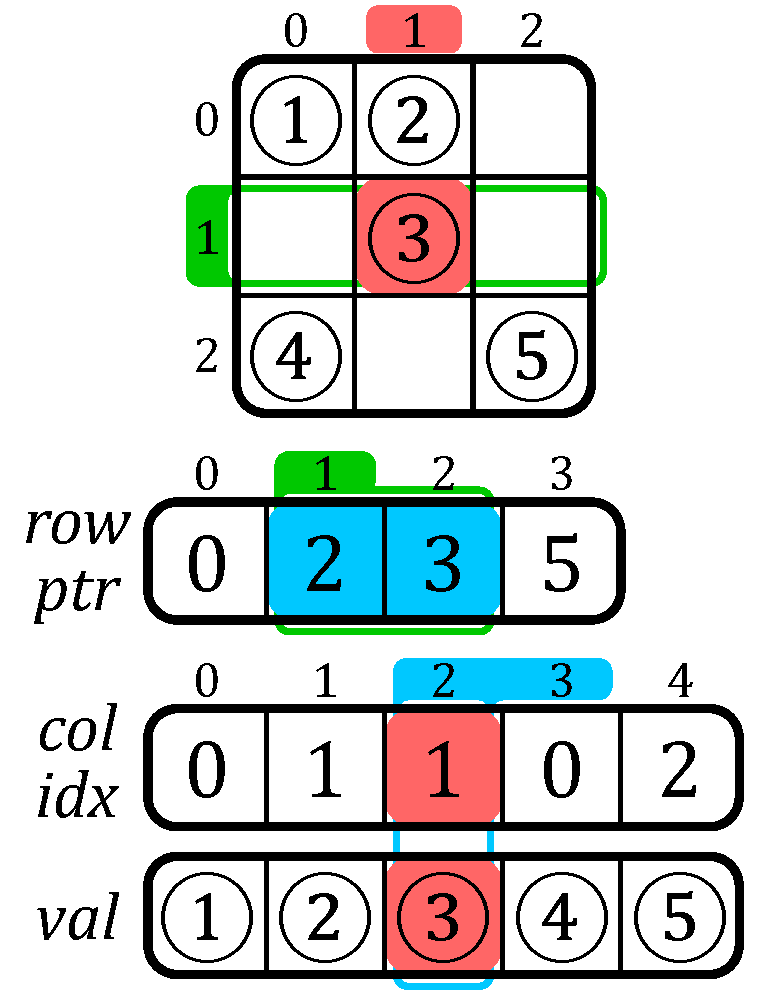
\includegraphics[width=0.8\linewidth]{Chapter_Background/Figures/PDF/SparseFormats/SpFormats_CSR.pdf}
        \caption{\acrshort{csr}}
        \label{fig:bg:FormatEx:CSR}
    \end{subfigure}
    \hfill
    \begin{subfigure}[t]{0.32\linewidth}
        \centering
        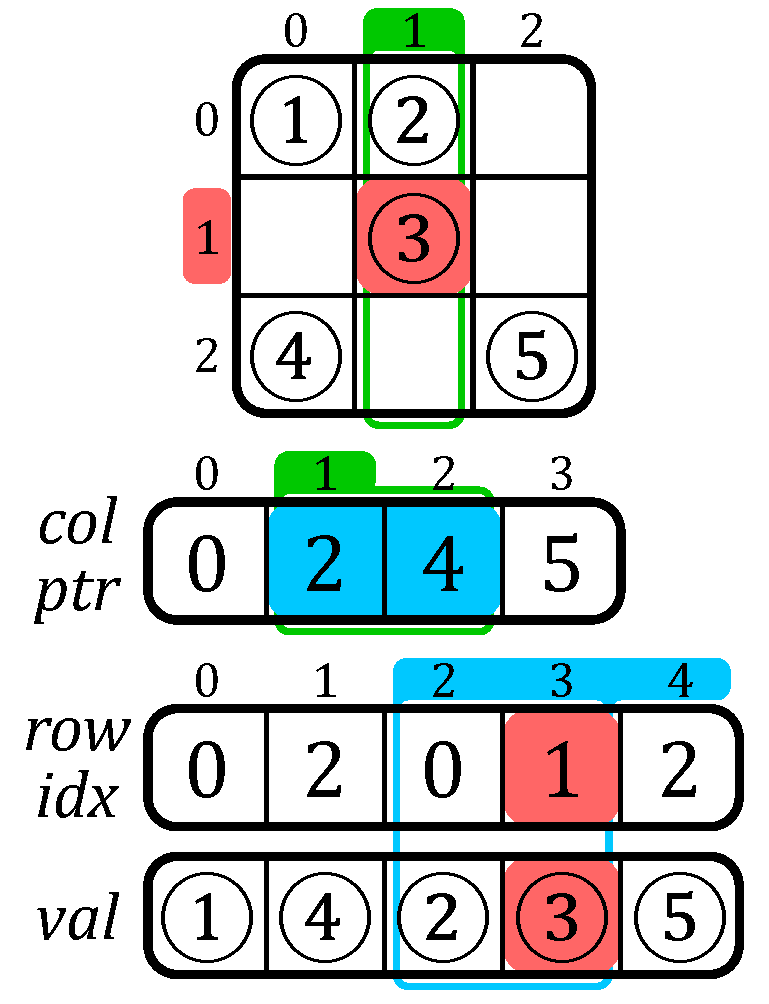
\includegraphics[width=0.8\linewidth]{Chapter_Background/Figures/PDF/SparseFormats/SpFormats_CSC.pdf}
        \caption{\acrshort{csc}}
        \label{fig:bg:FormatEx:CSC}
    \end{subfigure}
    \caption{Example of a Sparse Matrix in \acrshort{coo}, \acrshort{csr} and \acrshort{csc} Formats}
    \label{fig:bg:FormatEx}
\end{figure}

Many others classes of \glspl{spFormat} exists such as \acrfull{bcsr}, \acrfull{dia}, \acrfull{ell} and \acrfull{hyb}, which all have their own advantages depending on the matrix structure or the hardware setup.
Some details on these formats are mentioned in Appendix~\ref{app:sparse_formats}.

In general, there is many derivates from the above main categories of \glspl{spFormat}.
Ultimately, we can create any format we want depending of our needs and constraints in software and hardware.
Latter in this manuscript, we indeed use a custom \gls{spFormat} called \acrfull{bacsc} that is an extension of \acrshort{csc} for \gls{banded} matrices.
As shown in Figure~\ref{fig:bg:FormatEx:BaCSC}, we added extra information in the $ptr$ table to identify the beginning and end of the \gls{band}.
Indeed, three pointers instead of one are now needed per column, as shown with the example of column $2$ in \textit{yellow}.
The column is split in one in-\gls{band} (IB) region in the middle and two out-of-\gls{band} (OB) regions around.
The $ptr$ table size is thus extended to $3 \times M + 1$.
With this format, we can avoid the computational cost of identifying in which region non-zero elements are, while traversing the matrix, a feature we take advantage of in Chapter~\ref{cha:eval}.

\begin{figure}[htbp]
    \centering
    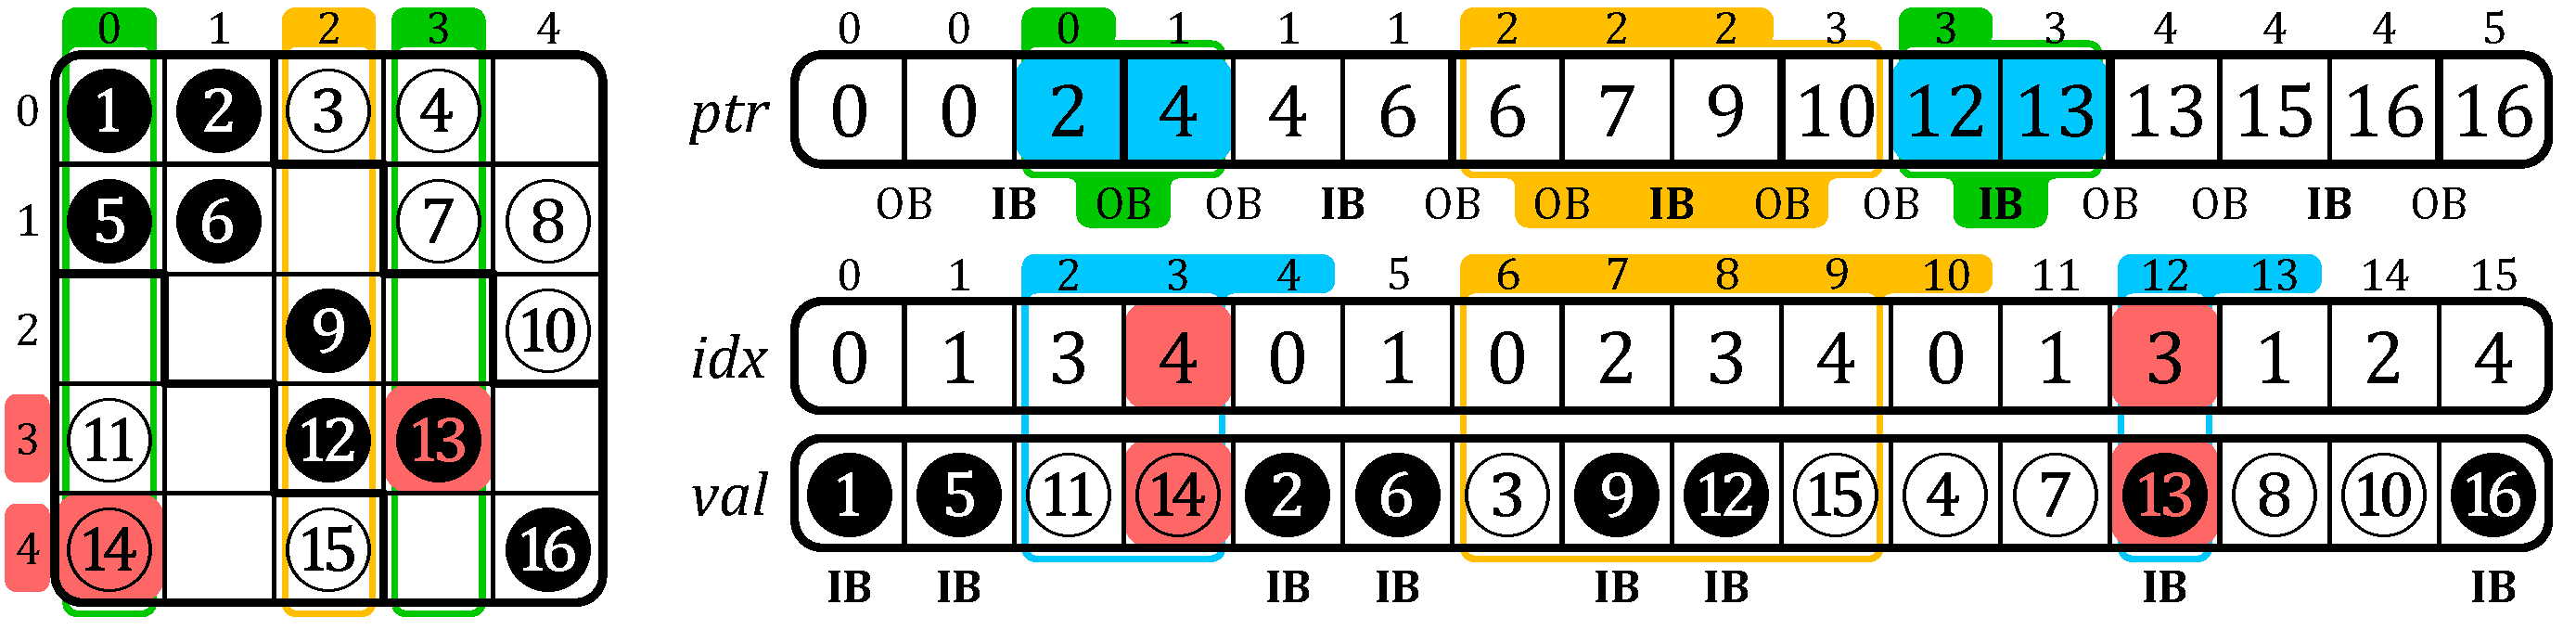
\includegraphics[width=\linewidth]{Chapter_Background/Figures/PDF/SparseFormats/SpFormats_BaCSC.pdf}
    \caption{Example of a Sparse Matrix in \acrshort{bacsc} Format}
    \label{fig:bg:FormatEx:BaCSC}
\end{figure}

\begin{highlight}{Definition}{LimeGreen}
    A \textbf{\gls{spFormat}} is a compression format for sparse matrices, which avoids storing zeros by using \gls{metadata}.
\end{highlight}

\begin{highlight}{Note}{SkyBlue}
    The mostly used \glspl{spFormat} are \acrshort{coo}, \acrshort{csr} and \acrshort{csc}.
\end{highlight}

\begin{highlight}{Conclusion}{Red}
    With the use of \glspl{spFormat}, it is possible to greatly \textbf{decrease memory footprints} while increasing the data dimensions.
    It allows great \textbf{flexibility} to manage data structure in software and hardware.
\end{highlight}